\begin{figure}[H]
    \par\noindent\rule{\textwidth}{0.4pt} \vspace{1em}
    \centering
    \begin{picture}(0,0)
        \put(-240,20){\small\textbf{(e)}}
    \end{picture}
    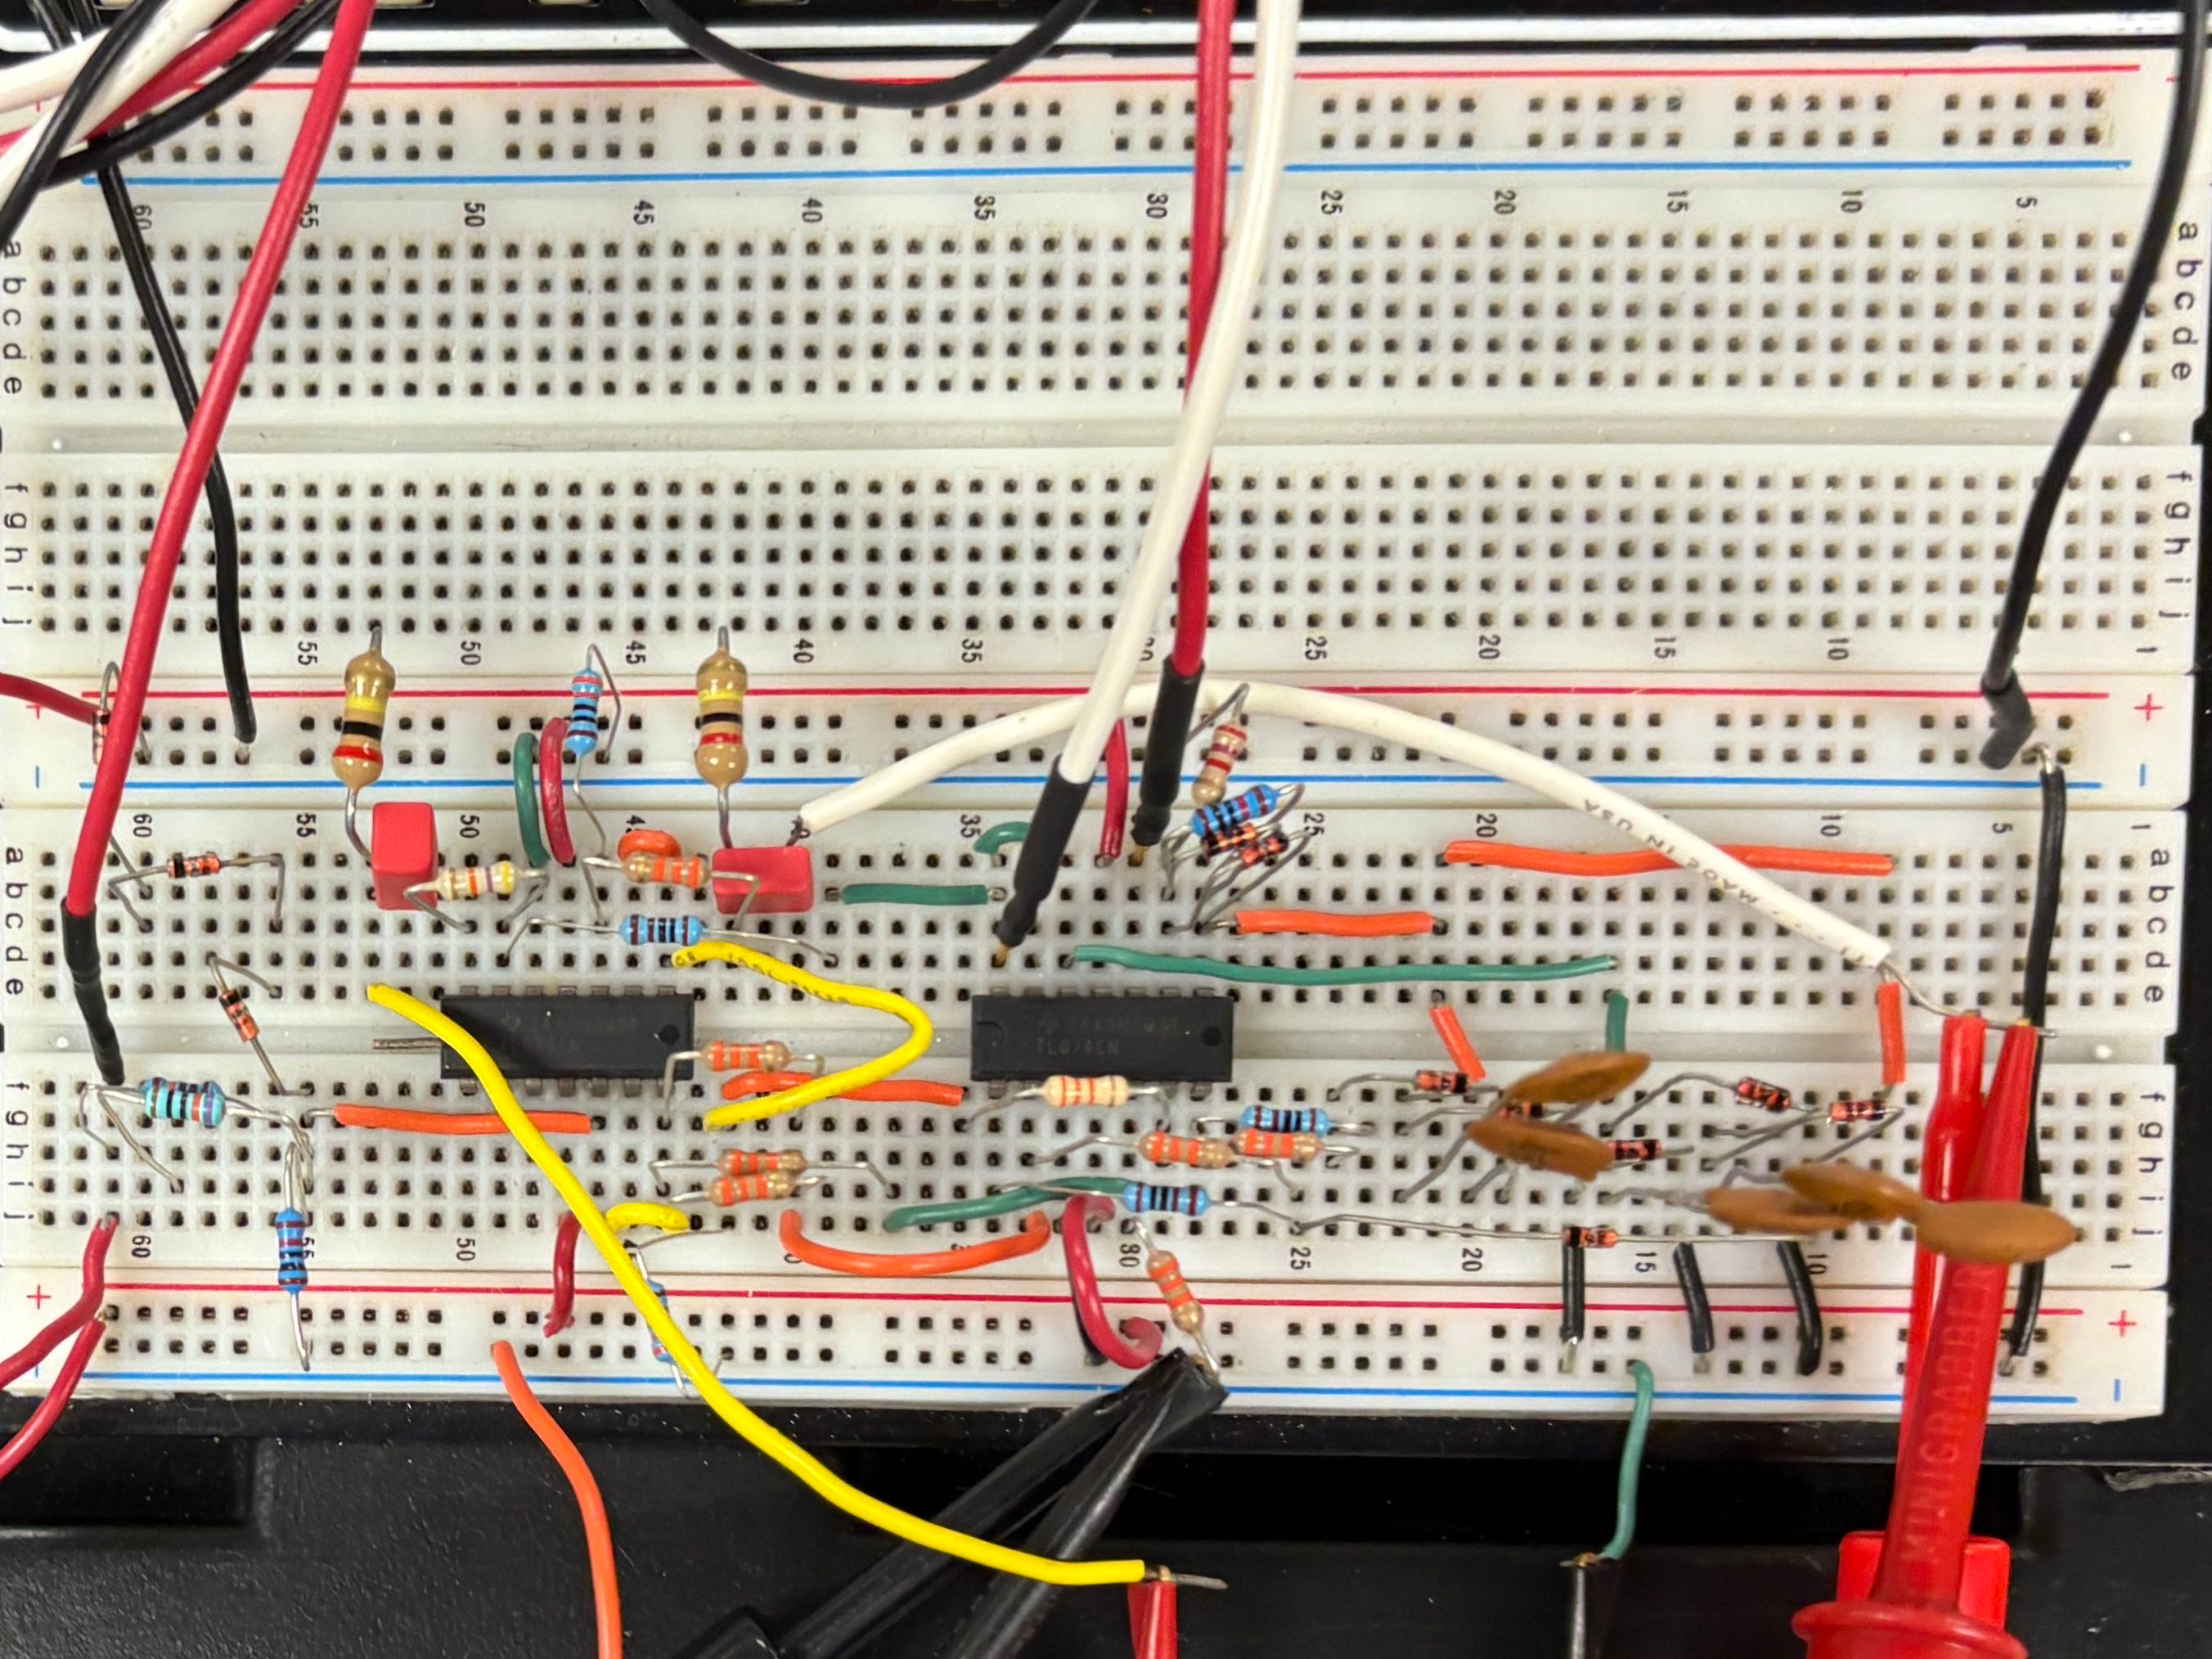
\includegraphics[width=0.8\textwidth]{../assets/breadboard.png}
    \caption{The circuit, implemented on breadboard. This may be modified to use the remaining op-amp on the bottom left to buffer the output for output to an amplifier.}
    \label{fig:breadboard}
    \par\noindent\rule{\textwidth}{0.4pt}
\end{figure}
